\section{Мета}
Вивчення організації та принципів роботи клавіатури та набуття практичних навичок управління мікропроцесором клавіатури.


\section{Завдання}
Відповідно до індивідуального завдання:
\begin{itemize}
    \item встановити відповідні період та затримку автоповтору;
    \item здійснити миготіння відповідного світлодіода.
\end{itemize}
Шляхом читання з порту 60h скан-коду визначити клавішу,
сканкод натискання якої збігається з номером студента в журналі.
Визначити сканкод віджимання цієї клавіши.
При визначенні скан-кодів можна скористатися алгоритмом, наведеним на рис. 4.2.

\section{Хід роботи}
\subsection{Код програми}
\lstinputlisting[language=Rust, style=colouredRust]{\codeDirectory/lab4/main.c}

\subsection{Результат роботи програми}
\begin{figure}[ht!]
    \centering
    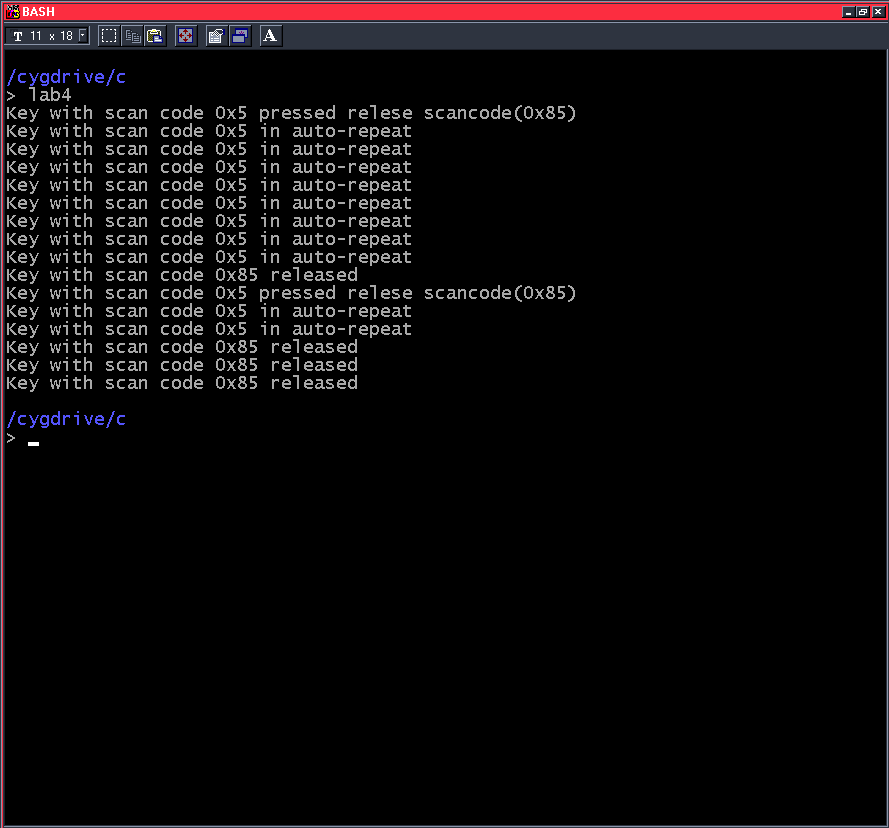
\includegraphics[width=0.9\textwidth]{\assetsDirectory/lab4.png}
    \caption{Результат роботи програми}
\end{figure}

\clearpage
\section{Висновки}
У процесі виконання практичної роботи було вивчено принципи функціонування клавіатури та здобуто практичні навички керування мікропроцесором клавіатури.
